% Created by tikzDevice version 0.12.3.1 on 2022-05-06 17:52:49
% !TEX encoding = UTF-8 Unicode
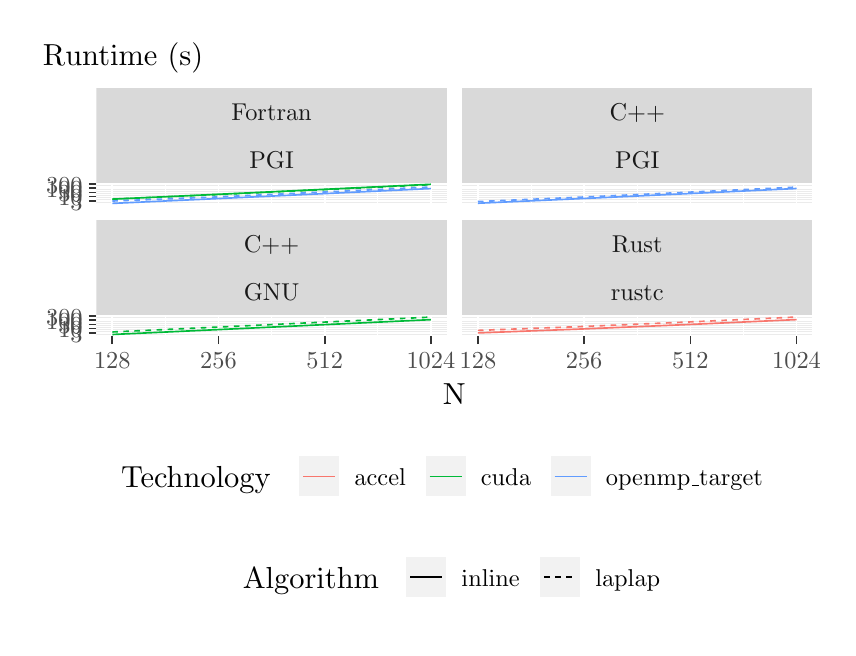
\begin{tikzpicture}[x=1pt,y=1pt]
\definecolor{fillColor}{RGB}{255,255,255}
\path[use as bounding box,fill=fillColor] (0,0) rectangle (289.08,216.81);
\begin{scope}
\path[clip] (  0.00,  0.00) rectangle (289.08,216.81);
\definecolor{drawColor}{RGB}{255,255,255}

\path[draw=drawColor,line width= 0.6pt,line join=round,line cap=round,fill=fillColor] (  0.00,  0.00) rectangle (289.08,216.81);
\end{scope}
\begin{scope}
\path[clip] ( 24.82,152.96) rectangle (151.45,160.55);
\definecolor{fillColor}{gray}{0.92}

\path[fill=fillColor] ( 24.82,152.96) rectangle (151.45,160.55);
\definecolor{drawColor}{RGB}{255,255,255}

\path[draw=drawColor,line width= 0.3pt,line join=round] ( 24.82,153.44) --
	(151.45,153.44);

\path[draw=drawColor,line width= 0.3pt,line join=round] ( 24.82,155.01) --
	(151.45,155.01);

\path[draw=drawColor,line width= 0.3pt,line join=round] ( 24.82,156.52) --
	(151.45,156.52);

\path[draw=drawColor,line width= 0.3pt,line join=round] ( 24.82,158.02) --
	(151.45,158.02);

\path[draw=drawColor,line width= 0.3pt,line join=round] ( 24.82,159.53) --
	(151.45,159.53);

\path[draw=drawColor,line width= 0.3pt,line join=round] ( 49.76,152.96) --
	( 49.76,160.55);

\path[draw=drawColor,line width= 0.3pt,line join=round] ( 88.14,152.96) --
	( 88.14,160.55);

\path[draw=drawColor,line width= 0.3pt,line join=round] (126.51,152.96) --
	(126.51,160.55);

\path[draw=drawColor,line width= 0.6pt,line join=round] ( 24.82,154.22) --
	(151.45,154.22);

\path[draw=drawColor,line width= 0.6pt,line join=round] ( 24.82,155.80) --
	(151.45,155.80);

\path[draw=drawColor,line width= 0.6pt,line join=round] ( 24.82,157.24) --
	(151.45,157.24);

\path[draw=drawColor,line width= 0.6pt,line join=round] ( 24.82,158.81) --
	(151.45,158.81);

\path[draw=drawColor,line width= 0.6pt,line join=round] ( 24.82,160.25) --
	(151.45,160.25);

\path[draw=drawColor,line width= 0.6pt,line join=round] ( 30.58,152.96) --
	( 30.58,160.55);

\path[draw=drawColor,line width= 0.6pt,line join=round] ( 68.95,152.96) --
	( 68.95,160.55);

\path[draw=drawColor,line width= 0.6pt,line join=round] (107.32,152.96) --
	(107.32,160.55);

\path[draw=drawColor,line width= 0.6pt,line join=round] (145.70,152.96) --
	(145.70,160.55);
\definecolor{drawColor}{RGB}{0,186,56}

\path[draw=drawColor,line width= 0.6pt,line join=round] ( 30.58,154.85) --
	( 68.95,156.60) --
	(107.32,158.40) --
	(145.70,160.21);
\definecolor{drawColor}{RGB}{97,156,255}

\path[draw=drawColor,line width= 0.6pt,line join=round] ( 30.58,153.31) --
	( 68.95,155.06) --
	(107.32,156.85) --
	(145.70,158.67);
\definecolor{drawColor}{RGB}{0,186,56}

\path[draw=drawColor,line width= 0.6pt,dash pattern=on 2pt off 2pt ,line join=round] ( 30.58,154.83) --
	( 68.95,156.52) --
	(107.32,158.28) --
	(145.70,160.08);
\definecolor{drawColor}{RGB}{97,156,255}

\path[draw=drawColor,line width= 0.6pt,dash pattern=on 2pt off 2pt ,line join=round] ( 30.58,154.17) --
	( 68.95,155.66) --
	(107.32,157.43) --
	(145.70,159.22);
\end{scope}
\begin{scope}
\path[clip] ( 24.82,105.25) rectangle (151.45,112.84);
\definecolor{fillColor}{gray}{0.92}

\path[fill=fillColor] ( 24.82,105.25) rectangle (151.45,112.84);
\definecolor{drawColor}{RGB}{255,255,255}

\path[draw=drawColor,line width= 0.3pt,line join=round] ( 24.82,105.73) --
	(151.45,105.73);

\path[draw=drawColor,line width= 0.3pt,line join=round] ( 24.82,107.30) --
	(151.45,107.30);

\path[draw=drawColor,line width= 0.3pt,line join=round] ( 24.82,108.81) --
	(151.45,108.81);

\path[draw=drawColor,line width= 0.3pt,line join=round] ( 24.82,110.31) --
	(151.45,110.31);

\path[draw=drawColor,line width= 0.3pt,line join=round] ( 24.82,111.82) --
	(151.45,111.82);

\path[draw=drawColor,line width= 0.3pt,line join=round] ( 49.76,105.25) --
	( 49.76,112.84);

\path[draw=drawColor,line width= 0.3pt,line join=round] ( 88.14,105.25) --
	( 88.14,112.84);

\path[draw=drawColor,line width= 0.3pt,line join=round] (126.51,105.25) --
	(126.51,112.84);

\path[draw=drawColor,line width= 0.6pt,line join=round] ( 24.82,106.51) --
	(151.45,106.51);

\path[draw=drawColor,line width= 0.6pt,line join=round] ( 24.82,108.09) --
	(151.45,108.09);

\path[draw=drawColor,line width= 0.6pt,line join=round] ( 24.82,109.53) --
	(151.45,109.53);

\path[draw=drawColor,line width= 0.6pt,line join=round] ( 24.82,111.10) --
	(151.45,111.10);

\path[draw=drawColor,line width= 0.6pt,line join=round] ( 24.82,112.54) --
	(151.45,112.54);

\path[draw=drawColor,line width= 0.6pt,line join=round] ( 30.58,105.25) --
	( 30.58,112.84);

\path[draw=drawColor,line width= 0.6pt,line join=round] ( 68.95,105.25) --
	( 68.95,112.84);

\path[draw=drawColor,line width= 0.6pt,line join=round] (107.32,105.25) --
	(107.32,112.84);

\path[draw=drawColor,line width= 0.6pt,line join=round] (145.70,105.25) --
	(145.70,112.84);
\definecolor{drawColor}{RGB}{0,186,56}

\path[draw=drawColor,line width= 0.6pt,line join=round] ( 30.58,105.94) --
	( 68.95,107.71) --
	(107.32,109.50) --
	(145.70,111.30);

\path[draw=drawColor,line width= 0.6pt,dash pattern=on 2pt off 2pt ,line join=round] ( 30.58,106.85) --
	( 68.95,108.63) --
	(107.32,110.42) --
	(145.70,112.22);
\end{scope}
\begin{scope}
\path[clip] (156.95,152.96) rectangle (283.58,160.55);
\definecolor{fillColor}{gray}{0.92}

\path[fill=fillColor] (156.95,152.96) rectangle (283.58,160.55);
\definecolor{drawColor}{RGB}{255,255,255}

\path[draw=drawColor,line width= 0.3pt,line join=round] (156.95,153.44) --
	(283.58,153.44);

\path[draw=drawColor,line width= 0.3pt,line join=round] (156.95,155.01) --
	(283.58,155.01);

\path[draw=drawColor,line width= 0.3pt,line join=round] (156.95,156.52) --
	(283.58,156.52);

\path[draw=drawColor,line width= 0.3pt,line join=round] (156.95,158.02) --
	(283.58,158.02);

\path[draw=drawColor,line width= 0.3pt,line join=round] (156.95,159.53) --
	(283.58,159.53);

\path[draw=drawColor,line width= 0.3pt,line join=round] (181.89,152.96) --
	(181.89,160.55);

\path[draw=drawColor,line width= 0.3pt,line join=round] (220.27,152.96) --
	(220.27,160.55);

\path[draw=drawColor,line width= 0.3pt,line join=round] (258.64,152.96) --
	(258.64,160.55);

\path[draw=drawColor,line width= 0.6pt,line join=round] (156.95,154.22) --
	(283.58,154.22);

\path[draw=drawColor,line width= 0.6pt,line join=round] (156.95,155.80) --
	(283.58,155.80);

\path[draw=drawColor,line width= 0.6pt,line join=round] (156.95,157.24) --
	(283.58,157.24);

\path[draw=drawColor,line width= 0.6pt,line join=round] (156.95,158.81) --
	(283.58,158.81);

\path[draw=drawColor,line width= 0.6pt,line join=round] (156.95,160.25) --
	(283.58,160.25);

\path[draw=drawColor,line width= 0.6pt,line join=round] (162.71,152.96) --
	(162.71,160.55);

\path[draw=drawColor,line width= 0.6pt,line join=round] (201.08,152.96) --
	(201.08,160.55);

\path[draw=drawColor,line width= 0.6pt,line join=round] (239.45,152.96) --
	(239.45,160.55);

\path[draw=drawColor,line width= 0.6pt,line join=round] (277.82,152.96) --
	(277.82,160.55);
\definecolor{drawColor}{RGB}{97,156,255}

\path[draw=drawColor,line width= 0.6pt,line join=round] (162.71,153.37) --
	(201.08,155.09) --
	(239.45,156.88) --
	(277.82,158.69);

\path[draw=drawColor,line width= 0.6pt,dash pattern=on 2pt off 2pt ,line join=round] (162.71,153.97) --
	(201.08,155.62) --
	(239.45,157.39) --
	(277.82,159.19);
\end{scope}
\begin{scope}
\path[clip] (156.95,105.25) rectangle (283.58,112.84);
\definecolor{fillColor}{gray}{0.92}

\path[fill=fillColor] (156.95,105.25) rectangle (283.58,112.84);
\definecolor{drawColor}{RGB}{255,255,255}

\path[draw=drawColor,line width= 0.3pt,line join=round] (156.95,105.73) --
	(283.58,105.73);

\path[draw=drawColor,line width= 0.3pt,line join=round] (156.95,107.30) --
	(283.58,107.30);

\path[draw=drawColor,line width= 0.3pt,line join=round] (156.95,108.81) --
	(283.58,108.81);

\path[draw=drawColor,line width= 0.3pt,line join=round] (156.95,110.31) --
	(283.58,110.31);

\path[draw=drawColor,line width= 0.3pt,line join=round] (156.95,111.82) --
	(283.58,111.82);

\path[draw=drawColor,line width= 0.3pt,line join=round] (181.89,105.25) --
	(181.89,112.84);

\path[draw=drawColor,line width= 0.3pt,line join=round] (220.27,105.25) --
	(220.27,112.84);

\path[draw=drawColor,line width= 0.3pt,line join=round] (258.64,105.25) --
	(258.64,112.84);

\path[draw=drawColor,line width= 0.6pt,line join=round] (156.95,106.51) --
	(283.58,106.51);

\path[draw=drawColor,line width= 0.6pt,line join=round] (156.95,108.09) --
	(283.58,108.09);

\path[draw=drawColor,line width= 0.6pt,line join=round] (156.95,109.53) --
	(283.58,109.53);

\path[draw=drawColor,line width= 0.6pt,line join=round] (156.95,111.10) --
	(283.58,111.10);

\path[draw=drawColor,line width= 0.6pt,line join=round] (156.95,112.54) --
	(283.58,112.54);

\path[draw=drawColor,line width= 0.6pt,line join=round] (162.71,105.25) --
	(162.71,112.84);

\path[draw=drawColor,line width= 0.6pt,line join=round] (201.08,105.25) --
	(201.08,112.84);

\path[draw=drawColor,line width= 0.6pt,line join=round] (239.45,105.25) --
	(239.45,112.84);

\path[draw=drawColor,line width= 0.6pt,line join=round] (277.82,105.25) --
	(277.82,112.84);
\definecolor{drawColor}{RGB}{248,118,109}

\path[draw=drawColor,line width= 0.6pt,line join=round] (162.71,106.51) --
	(201.08,107.96) --
	(239.45,109.57) --
	(277.82,111.32);

\path[draw=drawColor,line width= 0.6pt,dash pattern=on 2pt off 2pt ,line join=round] (162.71,107.42) --
	(201.08,108.84) --
	(239.45,110.49) --
	(277.82,112.24);
\end{scope}
\begin{scope}
\path[clip] ( 24.82,130.15) rectangle (151.45,147.46);
\definecolor{fillColor}{gray}{0.85}

\path[fill=fillColor] ( 24.82,130.15) rectangle (151.45,147.46);
\definecolor{drawColor}{gray}{0.10}

\node[text=drawColor,anchor=base,inner sep=0pt, outer sep=0pt, scale=  0.88] at ( 88.14,135.49) {C++};
\end{scope}
\begin{scope}
\path[clip] ( 24.82,112.84) rectangle (151.45,130.15);
\definecolor{fillColor}{gray}{0.85}

\path[fill=fillColor] ( 24.82,112.84) rectangle (151.45,130.15);
\definecolor{drawColor}{gray}{0.10}

\node[text=drawColor,anchor=base,inner sep=0pt, outer sep=0pt, scale=  0.88] at ( 88.14,118.18) {GNU};
\end{scope}
\begin{scope}
\path[clip] (156.95,130.15) rectangle (283.58,147.46);
\definecolor{fillColor}{gray}{0.85}

\path[fill=fillColor] (156.95,130.15) rectangle (283.58,147.46);
\definecolor{drawColor}{gray}{0.10}

\node[text=drawColor,anchor=base,inner sep=0pt, outer sep=0pt, scale=  0.88] at (220.27,135.49) {Rust};
\end{scope}
\begin{scope}
\path[clip] (156.95,112.84) rectangle (283.58,130.15);
\definecolor{fillColor}{gray}{0.85}

\path[fill=fillColor] (156.95,112.84) rectangle (283.58,130.15);
\definecolor{drawColor}{gray}{0.10}

\node[text=drawColor,anchor=base,inner sep=0pt, outer sep=0pt, scale=  0.88] at (220.27,118.18) {rustc};
\end{scope}
\begin{scope}
\path[clip] ( 24.82,177.86) rectangle (151.45,195.17);
\definecolor{fillColor}{gray}{0.85}

\path[fill=fillColor] ( 24.82,177.86) rectangle (151.45,195.17);
\definecolor{drawColor}{gray}{0.10}

\node[text=drawColor,anchor=base,inner sep=0pt, outer sep=0pt, scale=  0.88] at ( 88.14,183.20) {Fortran};
\end{scope}
\begin{scope}
\path[clip] ( 24.82,160.55) rectangle (151.45,177.86);
\definecolor{fillColor}{gray}{0.85}

\path[fill=fillColor] ( 24.82,160.55) rectangle (151.45,177.86);
\definecolor{drawColor}{gray}{0.10}

\node[text=drawColor,anchor=base,inner sep=0pt, outer sep=0pt, scale=  0.88] at ( 88.14,165.89) {PGI};
\end{scope}
\begin{scope}
\path[clip] (156.95,177.86) rectangle (283.58,195.17);
\definecolor{fillColor}{gray}{0.85}

\path[fill=fillColor] (156.95,177.86) rectangle (283.58,195.17);
\definecolor{drawColor}{gray}{0.10}

\node[text=drawColor,anchor=base,inner sep=0pt, outer sep=0pt, scale=  0.88] at (220.27,183.20) {C++};
\end{scope}
\begin{scope}
\path[clip] (156.95,160.55) rectangle (283.58,177.86);
\definecolor{fillColor}{gray}{0.85}

\path[fill=fillColor] (156.95,160.55) rectangle (283.58,177.86);
\definecolor{drawColor}{gray}{0.10}

\node[text=drawColor,anchor=base,inner sep=0pt, outer sep=0pt, scale=  0.88] at (220.27,165.89) {PGI};
\end{scope}
\begin{scope}
\path[clip] (  0.00,  0.00) rectangle (289.08,216.81);
\definecolor{drawColor}{gray}{0.20}

\path[draw=drawColor,line width= 0.6pt,line join=round] ( 30.58,102.50) --
	( 30.58,105.25);

\path[draw=drawColor,line width= 0.6pt,line join=round] ( 68.95,102.50) --
	( 68.95,105.25);

\path[draw=drawColor,line width= 0.6pt,line join=round] (107.32,102.50) --
	(107.32,105.25);

\path[draw=drawColor,line width= 0.6pt,line join=round] (145.70,102.50) --
	(145.70,105.25);
\end{scope}
\begin{scope}
\path[clip] (  0.00,  0.00) rectangle (289.08,216.81);
\definecolor{drawColor}{gray}{0.30}

\node[text=drawColor,anchor=base,inner sep=0pt, outer sep=0pt, scale=  0.88] at ( 30.58, 93.67) {128};

\node[text=drawColor,anchor=base,inner sep=0pt, outer sep=0pt, scale=  0.88] at ( 68.95, 93.67) {256};

\node[text=drawColor,anchor=base,inner sep=0pt, outer sep=0pt, scale=  0.88] at (107.32, 93.67) {512};

\node[text=drawColor,anchor=base,inner sep=0pt, outer sep=0pt, scale=  0.88] at (145.70, 93.67) {1024};
\end{scope}
\begin{scope}
\path[clip] (  0.00,  0.00) rectangle (289.08,216.81);
\definecolor{drawColor}{gray}{0.20}

\path[draw=drawColor,line width= 0.6pt,line join=round] (162.71,102.50) --
	(162.71,105.25);

\path[draw=drawColor,line width= 0.6pt,line join=round] (201.08,102.50) --
	(201.08,105.25);

\path[draw=drawColor,line width= 0.6pt,line join=round] (239.45,102.50) --
	(239.45,105.25);

\path[draw=drawColor,line width= 0.6pt,line join=round] (277.82,102.50) --
	(277.82,105.25);
\end{scope}
\begin{scope}
\path[clip] (  0.00,  0.00) rectangle (289.08,216.81);
\definecolor{drawColor}{gray}{0.30}

\node[text=drawColor,anchor=base,inner sep=0pt, outer sep=0pt, scale=  0.88] at (162.71, 93.67) {128};

\node[text=drawColor,anchor=base,inner sep=0pt, outer sep=0pt, scale=  0.88] at (201.08, 93.67) {256};

\node[text=drawColor,anchor=base,inner sep=0pt, outer sep=0pt, scale=  0.88] at (239.45, 93.67) {512};

\node[text=drawColor,anchor=base,inner sep=0pt, outer sep=0pt, scale=  0.88] at (277.82, 93.67) {1024};
\end{scope}
\begin{scope}
\path[clip] (  0.00,  0.00) rectangle (289.08,216.81);
\definecolor{drawColor}{gray}{0.30}

\node[text=drawColor,anchor=base east,inner sep=0pt, outer sep=0pt, scale=  0.88] at ( 19.87,150.91) {3};

\node[text=drawColor,anchor=base east,inner sep=0pt, outer sep=0pt, scale=  0.88] at ( 19.87,152.48) {10};

\node[text=drawColor,anchor=base east,inner sep=0pt, outer sep=0pt, scale=  0.88] at ( 19.87,153.92) {30};

\node[text=drawColor,anchor=base east,inner sep=0pt, outer sep=0pt, scale=  0.88] at ( 19.87,155.49) {100};

\node[text=drawColor,anchor=base east,inner sep=0pt, outer sep=0pt, scale=  0.88] at ( 19.87,156.93) {300};
\end{scope}
\begin{scope}
\path[clip] (  0.00,  0.00) rectangle (289.08,216.81);
\definecolor{drawColor}{gray}{0.20}

\path[draw=drawColor,line width= 0.6pt,line join=round] ( 22.07,154.22) --
	( 24.82,154.22);

\path[draw=drawColor,line width= 0.6pt,line join=round] ( 22.07,155.80) --
	( 24.82,155.80);

\path[draw=drawColor,line width= 0.6pt,line join=round] ( 22.07,157.24) --
	( 24.82,157.24);

\path[draw=drawColor,line width= 0.6pt,line join=round] ( 22.07,158.81) --
	( 24.82,158.81);

\path[draw=drawColor,line width= 0.6pt,line join=round] ( 22.07,160.25) --
	( 24.82,160.25);
\end{scope}
\begin{scope}
\path[clip] (  0.00,  0.00) rectangle (289.08,216.81);
\definecolor{drawColor}{gray}{0.30}

\node[text=drawColor,anchor=base east,inner sep=0pt, outer sep=0pt, scale=  0.88] at ( 19.87,103.20) {3};

\node[text=drawColor,anchor=base east,inner sep=0pt, outer sep=0pt, scale=  0.88] at ( 19.87,104.77) {10};

\node[text=drawColor,anchor=base east,inner sep=0pt, outer sep=0pt, scale=  0.88] at ( 19.87,106.21) {30};

\node[text=drawColor,anchor=base east,inner sep=0pt, outer sep=0pt, scale=  0.88] at ( 19.87,107.78) {100};

\node[text=drawColor,anchor=base east,inner sep=0pt, outer sep=0pt, scale=  0.88] at ( 19.87,109.22) {300};
\end{scope}
\begin{scope}
\path[clip] (  0.00,  0.00) rectangle (289.08,216.81);
\definecolor{drawColor}{gray}{0.20}

\path[draw=drawColor,line width= 0.6pt,line join=round] ( 22.07,106.51) --
	( 24.82,106.51);

\path[draw=drawColor,line width= 0.6pt,line join=round] ( 22.07,108.09) --
	( 24.82,108.09);

\path[draw=drawColor,line width= 0.6pt,line join=round] ( 22.07,109.53) --
	( 24.82,109.53);

\path[draw=drawColor,line width= 0.6pt,line join=round] ( 22.07,111.10) --
	( 24.82,111.10);

\path[draw=drawColor,line width= 0.6pt,line join=round] ( 22.07,112.54) --
	( 24.82,112.54);
\end{scope}
\begin{scope}
\path[clip] (  0.00,  0.00) rectangle (289.08,216.81);
\definecolor{drawColor}{RGB}{0,0,0}

\node[text=drawColor,anchor=base,inner sep=0pt, outer sep=0pt, scale=  1.10] at (154.20, 80.75) {N};
\end{scope}
\begin{scope}
\path[clip] (  0.00,  0.00) rectangle (289.08,216.81);
\definecolor{fillColor}{RGB}{255,255,255}

\path[fill=fillColor] ( 28.25, 41.95) rectangle (280.16, 67.41);
\end{scope}
\begin{scope}
\path[clip] (  0.00,  0.00) rectangle (289.08,216.81);
\definecolor{drawColor}{RGB}{0,0,0}

\node[text=drawColor,anchor=base west,inner sep=0pt, outer sep=0pt, scale=  1.10] at ( 33.75, 50.53) {Technology};
\end{scope}
\begin{scope}
\path[clip] (  0.00,  0.00) rectangle (289.08,216.81);
\definecolor{fillColor}{gray}{0.95}

\path[fill=fillColor] ( 98.13, 47.45) rectangle (112.59, 61.91);
\end{scope}
\begin{scope}
\path[clip] (  0.00,  0.00) rectangle (289.08,216.81);
\definecolor{drawColor}{RGB}{248,118,109}

\path[draw=drawColor,line width= 0.6pt,line join=round] ( 99.58, 54.68) -- (111.14, 54.68);
\end{scope}
\begin{scope}
\path[clip] (  0.00,  0.00) rectangle (289.08,216.81);
\definecolor{fillColor}{gray}{0.95}

\path[fill=fillColor] (143.82, 47.45) rectangle (158.27, 61.91);
\end{scope}
\begin{scope}
\path[clip] (  0.00,  0.00) rectangle (289.08,216.81);
\definecolor{drawColor}{RGB}{0,186,56}

\path[draw=drawColor,line width= 0.6pt,line join=round] (145.26, 54.68) -- (156.83, 54.68);
\end{scope}
\begin{scope}
\path[clip] (  0.00,  0.00) rectangle (289.08,216.81);
\definecolor{fillColor}{gray}{0.95}

\path[fill=fillColor] (188.97, 47.45) rectangle (203.42, 61.91);
\end{scope}
\begin{scope}
\path[clip] (  0.00,  0.00) rectangle (289.08,216.81);
\definecolor{drawColor}{RGB}{97,156,255}

\path[draw=drawColor,line width= 0.6pt,line join=round] (190.41, 54.68) -- (201.97, 54.68);
\end{scope}
\begin{scope}
\path[clip] (  0.00,  0.00) rectangle (289.08,216.81);
\definecolor{drawColor}{RGB}{0,0,0}

\node[text=drawColor,anchor=base west,inner sep=0pt, outer sep=0pt, scale=  0.88] at (118.09, 51.36) {accel};
\end{scope}
\begin{scope}
\path[clip] (  0.00,  0.00) rectangle (289.08,216.81);
\definecolor{drawColor}{RGB}{0,0,0}

\node[text=drawColor,anchor=base west,inner sep=0pt, outer sep=0pt, scale=  0.88] at (163.77, 51.36) {cuda};
\end{scope}
\begin{scope}
\path[clip] (  0.00,  0.00) rectangle (289.08,216.81);
\definecolor{drawColor}{RGB}{0,0,0}

\node[text=drawColor,anchor=base west,inner sep=0pt, outer sep=0pt, scale=  0.88] at (208.92, 51.36) {openmp{\_{}}target};
\end{scope}
\begin{scope}
\path[clip] (  0.00,  0.00) rectangle (289.08,216.81);
\definecolor{fillColor}{RGB}{255,255,255}

\path[fill=fillColor] ( 72.24,  5.50) rectangle (236.16, 30.95);
\end{scope}
\begin{scope}
\path[clip] (  0.00,  0.00) rectangle (289.08,216.81);
\definecolor{drawColor}{RGB}{0,0,0}

\node[text=drawColor,anchor=base west,inner sep=0pt, outer sep=0pt, scale=  1.10] at ( 77.74, 14.08) {Algorithm};
\end{scope}
\begin{scope}
\path[clip] (  0.00,  0.00) rectangle (289.08,216.81);
\definecolor{fillColor}{gray}{0.95}

\path[fill=fillColor] (136.80, 11.00) rectangle (151.26, 25.45);
\end{scope}
\begin{scope}
\path[clip] (  0.00,  0.00) rectangle (289.08,216.81);
\definecolor{drawColor}{RGB}{0,0,0}

\path[draw=drawColor,line width= 0.6pt,line join=round] (138.25, 18.23) -- (149.81, 18.23);
\end{scope}
\begin{scope}
\path[clip] (  0.00,  0.00) rectangle (289.08,216.81);
\definecolor{fillColor}{gray}{0.95}

\path[fill=fillColor] (185.15, 11.00) rectangle (199.60, 25.45);
\end{scope}
\begin{scope}
\path[clip] (  0.00,  0.00) rectangle (289.08,216.81);
\definecolor{drawColor}{RGB}{0,0,0}

\path[draw=drawColor,line width= 0.6pt,dash pattern=on 2pt off 2pt ,line join=round] (186.60, 18.23) -- (198.16, 18.23);
\end{scope}
\begin{scope}
\path[clip] (  0.00,  0.00) rectangle (289.08,216.81);
\definecolor{drawColor}{RGB}{0,0,0}

\node[text=drawColor,anchor=base west,inner sep=0pt, outer sep=0pt, scale=  0.88] at (156.76, 14.91) {inline};
\end{scope}
\begin{scope}
\path[clip] (  0.00,  0.00) rectangle (289.08,216.81);
\definecolor{drawColor}{RGB}{0,0,0}

\node[text=drawColor,anchor=base west,inner sep=0pt, outer sep=0pt, scale=  0.88] at (205.10, 14.91) {laplap};
\end{scope}
\begin{scope}
\path[clip] (  0.00,  0.00) rectangle (289.08,216.81);
\definecolor{drawColor}{RGB}{0,0,0}

\node[text=drawColor,anchor=base west,inner sep=0pt, outer sep=0pt, scale=  1.10] at (  5.50,203.01) {Runtime (s)};
\end{scope}
\end{tikzpicture}
